\begin{abox}
	Statistical Mechanics 
	\end{abox}
\begin{enumerate}
\item In a system comprising of $N$ distinguishable particles, each particle may occupy any of 20 distinct states. The maximum value of the entropy per particle is nearest to (take ln20 as 3 )
\begin{tasks}(4)
\task[\textbf{A.}] $20 k_{B}$
\task[\textbf{B.}]  $3 k_{B}$
\task[\textbf{C.}] $10(\ln 2) k_{B}$
\task[\textbf{D.}] $20(\ln 2) k_{B}$
\end{tasks}
\begin{answer}
$$\begin{aligned}
\text{	For $N$ particles; }\Omega&=20^{N} .\\
S&=k_{B} \ln \Omega=k_{B} \ln 20^{N}=N k_{B} \ln 20 \\ \frac{S}{N}&=k_{B} \ln 20 \approx 3 k_{B} \quad \because \ln 20 \approx 3
\end{aligned}$$
So the correct answer is \textbf{Option (B)}
\end{answer}
	\item A particle hops on a one-dimensional lattice with lattice spacing $a$. The probability of the particle to hop to the neighboring site to its right is $p$, while the corresponding probability to hop to the left is $q=1-p$. The root-mean squared deviation $\Delta x=\sqrt{\left\langle x^{2}\right\rangle-\langle x\rangle^{2}}$ in displacement after $N$ steps, is
\begin{figure}[H]
\centering
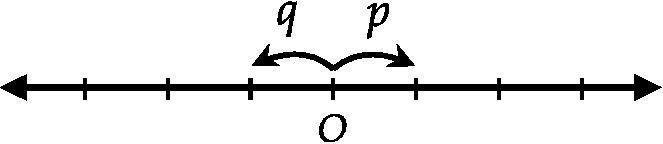
\includegraphics[height=1.1cm,width=6.5cm]{SP-1}
\end{figure}
\begin{tasks}(4)
\task[\textbf{A.}] $a \sqrt{N p q}$
\task[\textbf{B.}] $a N \sqrt{p q}$
\task[\textbf{C.}] $2 a \sqrt{N p q}$
\task[\textbf{D.}] $a \sqrt{N}$
\end{tasks}
\begin{answer}
$$\begin{aligned}	
\text{The standard deviation of Binomial distribution $=\sqrt{N p q}$}\\
\text{Step size } &=2 a\quad (\mathrm{L} \& \mathrm{R})\\
\text{Mean square displacement }&=2 a \sqrt{N p q}
\end{aligned}$$	
So the correct answer is \textbf{Option (C)}
\end{answer}

	\item In a system of $N$ distinguishable particles, each particle can be in one of two states with energies 0 and $-E$, respectively. The mean energy of the system at temperature $T$ is
\begin{tasks}(2)
\task[\textbf{A.}] $-\frac{1}{2} N\left(1+e^{\varepsilon / k_{B} T}\right)$
\task[\textbf{B.}] $-N E\left(1+e^{\delta / k_{B} T}\right)$
\task[\textbf{C.}] $-\frac{1}{2} N E$
\task[\textbf{D.}] $\frac{-N E}{1+e^{-E / k_{B} T}}$
\end{tasks}
\begin{answer}
$$\begin{aligned}	
\text{For one particle system}&\\
\langle E\rangle&=\frac{0 \times e^{\frac{-0}{k_{B} T}}+(-E) e^{+E / k_{B} T}}{e^{-0 / k_{B} T}+e^{E / k_{B} T}}\\&=\frac{-E e^{E / k_{B} T}}{1+e^{E / k_{B} T}}\\&=\frac{-E}{e^{-E / k_{k} T}+1}\\ \langle E\rangle&=\frac{-N E}{1+e^{-E / k_{B} T}}
\end{aligned}$$	
So the correct answer is \textbf{Option (D)}
\end{answer}
	

\item 	A system has two energy levels with energies $\varepsilon$ and $2 \varepsilon .$ The lower level is 4 -fold degenerate while the upper level is doubly degenerate. If there are $N$ non-interacting classical particles in the system, which is in thermodynamic equilibrium at a temperature $T$, the fraction of particles in the upper level is
\begin{tasks}(2)
\task[\textbf{A.}] $\frac{1}{1+e^{\varepsilon / k_{B} T}}$
\task[\textbf{B.}] $\frac{1}{1+2 e^{\varepsilon / k_{B} T}}$
\task[\textbf{C.}] $\frac{1}{2 e^{\varepsilon / k_{B} T}+4 e^{2 \varepsilon / k_{B} T}}$
\task[\textbf{D.}] $\frac{1}{2 e^{\varepsilon / k_{B} T}-4 e^{2 \varepsilon / k_{B} T}}$
\end{tasks}
\begin{answer}
$$\begin{aligned}	
\text{Partition function }Z&=4 e^{-\epsilon / k T}+2 e^{-\epsilon / k T} \\
 P(2 \varepsilon)&=\frac{2 e^{-2 \in / k T}}{4 e^{-\epsilon / k T}+2 e^{-2 \varepsilon / k T}}\\&=\frac{1}{1+2 e^{\epsilon / k T}}
\end{aligned}$$	
So the correct answer is \textbf{Option (B)}
\end{answer}

	\item Consider a system whose three energy levels are given by $0, \varepsilon$ and $2 \varepsilon$. The energy level $\varepsilon$ is two-fold degenerate and the other two are non-degenerate. The partition function of the system with $\beta=\frac{1}{k_{B} T}$ is given by
\begin{tasks}(2)
\task[\textbf{A.}] $1+2 e^{-\beta \varepsilon}$
\task[\textbf{B.}] $2 e^{-\beta \varepsilon}+e^{-2 \beta \varepsilon}$
\task[\textbf{C.}] $\left(1+e^{-\beta \varepsilon}\right)^{2}$
\task[\textbf{D.}] $1+e^{-\beta \varepsilon}+e^{-2 \beta \varepsilon}$
\end{tasks}
\begin{answer}
$$\begin{aligned}	
E_{1}&=0, E_{2}=\varepsilon, E_{3}=2 \varepsilon ; g_{1}=1, g_{2}=2, g_{3}=1\\&\text{ where} g_{1}, g_{2}\text{ and }g_{3}\text{ are degeneracy}\\
\text{	The partition function }Z&=g_{1} e^{-\beta \cdot E_{1}}+g_{2} e^{-\beta \cdot E_{2}}+g_{3} e^{-\beta \cdot E_{3}}\\&=1+2 e^{-\beta c}+e^{-\beta 2 \varepsilon}\\&=\left(1+e^{-\beta \epsilon}\right)^{2}
\end{aligned}$$	
So the correct answer is \textbf{Option (C)}
\end{answer}
	\item Consider a linear collection of $N$ independent spin $1 / 2$ particles, each at a fixed location. The entropy of this system is $(k$ is the Boltzmann constant)
\begin{tasks}(4)
\task[\textbf{A.}] Zero
\task[\textbf{B.}]  $N k$
\task[\textbf{C.}]  $\frac{1}{2} N k$
\task[\textbf{D.}] $N k \ln (2)$
\end{tasks}
\begin{answer}
$$	\begin{aligned}
\text{There are two microstates }&\text{possible for spin $\frac{1}{2}$ particle,}\\ 
\text{ so entropy is given by $N k \ln (2)$}&
\end{aligned}$$
So the correct answer is \textbf{Option (D)}
\end{answer}
\item A system consists of $N$ number of particles, $N>1 .$ Each particle can have only one of the two energies $E_{1}$ or $E_{1}+\varepsilon(\varepsilon>0) .$ If the system is in equilibrium at a temperature $T$ the average number of particles with energy $E_{1}$ is
\begin{tasks}(4)
\task[\textbf{A.}] $\frac{N}{2}$
\task[\textbf{B.}] $\frac{N}{e^{\varepsilon / k T}+1}$ 
\task[\textbf{C.}] $\frac{N}{e^{-\varepsilon / k T}+1}$
\task[\textbf{D.}] $N e^{\frac{-\varepsilon}{k T}}$
\end{tasks}
\begin{answer}
	$$\begin{aligned}
	\langle N\rangle&=N e^{\frac{-\left(E_{2}-E_{1}\right)}{k T}}\\
	&=N e^{\frac{-\left[\left(E_{1}+\varepsilon\right)-E_{1}\right]}{k T}} \\ 
	\langle N\rangle& =N e^{\frac{-\varepsilon}{k T}}
	\end{aligned}$$

Correct answer is \textbf{option (D)}
\end{answer}
\item The entropy of a gas containing $N$ particles enclosed in a volume $V$ is given by $S=N k_{B} \ln \left(\frac{a V E^{3 / 2}}{N^{5 / 2}}\right)$
where $E$ is the total energy, $a$ is a constant and $k_{B}$ is the Boltzmann constant. The chemical potential $\mu$ of the system at a temperature $T$ is given by
\begin{answer}
	$$\begin{aligned}
	\mu=-T\left(\frac{\partial S}{\partial N}\right)_{V, E}&=-T k_{B} \ln \left(\frac{a V E^{3 / 2}}{N^{5 / 2}}\right)-T k_{B} N \cdot \frac{N^{5 / 2}}{\rho V E^{3 / 2}} \cdot \rho V E^{3 / 2}\left(-\frac{5}{2} N^{-7 / 2}\right)\\
	&=-T k_{B} \ln \left(\frac{a V E^{3 / 2}}{N^{5 / 2}}\right)+\frac{5}{2} k_{B} T\\
	&=-k_{B} T\left[\ln \left(\frac{a V E^{3 / 2}}{N^{5 / 2}}\right)-\frac{5}{2}\right]
	\end{aligned}$$
\end{answer}
	
\item A collection of $N$ two-level systems with energies 0 and $E>0$ is in thermal
equilibrium at temperature $T$. For $T \rightarrow \infty$, the specific heat approaches to,
\begin{tasks}(4)
	\task[\textbf{A.}] 0
	\task[\textbf{B.}] $N k_{B}$
	\task[\textbf{C.}] $\frac{3 N k_{B}}{2}$
	\task[\textbf{D.}] $\infty$
\end{tasks}
\begin{answer}
	$$\begin{aligned}	
	Z&=\sum e^{-\beta E_{i}}=e^{-\beta \times 0}+e^{-\beta E_{i}} \Rightarrow Z\\&=1+e^{-\beta E} \Rightarrow \ln z\\&=\ln \left(1+e^{-\beta E}\right)\\
	U&=\langle E\rangle=-\frac{\partial}{\partial \beta} \ln z\\&=-\frac{\partial}{\partial \beta} \ln \left(1+e^{-\beta E}\right)\\&=-\frac{1}{1+e^{-\beta E}} \times e^{-\beta E}(-E)\\&=\frac{E e^{-\beta E}}{1+e^{-\beta E}}\\
	\text{Now},\left(\frac{\partial U}{\partial T}\right)_{V}&=C_{V}\\
	&=\frac{\partial}{\partial T}\left(\frac{E e^{-\frac{E}{k T}}}{1+e^{-\frac{E}{k T}}}\right)\\
	\Rightarrow C_{V}&=\frac{\left(\frac{E^{2}}{k T^{2}} e^{\frac{-E}{k T}}+\frac{E^{2}}{k T^{2}} e^{\frac{-2 E}{k T}}-\frac{E^{2}}{k T^{2}} e^{\frac{-2 E}{k T}}\right)}{\left(1+e^{\frac{-E}{k T}}\right)^{2}} \Rightarrow C_{V}\\
	&=\left.\frac{\frac{E^{2}}{k T^{2}} e^{\frac{-E}{k T}}}{\left(1+e^{\frac{-E}{k T}}\right)^{2}} \Rightarrow C_{V}\right|_{T \rightarrow \infty}=0
	\end{aligned}$$	
	So the correct answer is \textbf{Option (A)}
\end{answer}
\item Which among the following sets of Maxwell relations is correct? (U-internal energy, H-enthalpy, A-Helmholtz free energy and G-Gibbs free energy)
{	\exyear{GATE 2010}}
\begin{tasks}(2)
	\task[\textbf{A.}] $T=\left(\frac{\partial U}{\partial V}\right)_{S}$ and $P=\left(\frac{\partial U}{\partial S}\right)_{V}$
	\task[\textbf{B.}] $V=\left(\frac{\partial H}{\partial P}\right)_{S}$ and $T=\left(\frac{\partial H}{\partial S}\right)_{P}$
	\task[\textbf{C.}]  $P=-\left(\frac{\partial G}{\partial V}\right)_{T}$ and $V=\left(\frac{\partial G}{\partial P}\right)_{s}$
	\task[\textbf{D.}] $P=-\left(\frac{\partial A}{\partial S}\right)_{T}$ and $S=\left(\frac{\partial A}{\partial P}\right)_{V}$
\end{tasks}
\begin{answer}
	$$\begin{aligned}	
	d H&=T d S+V d P \Rightarrow\left(\frac{\partial H}{\partial S}\right)_{P}\\&=T,\left(\frac{\partial H}{\partial P}\right)_{S}=V
	\end{aligned}$$	
	So the correct answer is \textbf{Option (B)}
\end{answer}
\item The internal energy $E$ of a system is given by $E=\frac{b S^{3}}{V N}$, where $b$ is a constant and other symbols have their usual meaning. The temperature of this system is equal to

\begin{tasks}(4)
\task[\textbf{A.}] $\frac{b S^{2}}{V N}$
\task[\textbf{B.}] $\frac{3 b S^{2}}{V N}$
\task[\textbf{C.}]  $\frac{b S^{3}}{V^{2} N}$
\task[\textbf{D.}] $\left(\frac{S}{N}\right)^{2}$
\end{tasks}
\begin{answer}
$$\begin{aligned}	
T d S&=d E+P d V \Rightarrow d E\\&=T d S-P d V \\\left(\frac{\partial E}{\partial S}\right)_{V}&=T \Rightarrow T=\frac{3 b S^{2}}{V N}
\end{aligned}$$	
So the correct answer is \textbf{Option (B)}
\end{answer}
\item A vessel has two compartments of volume $V_{1}$ and $V_{2}$, containing an ideal gas at pressures $p_{1}$ and $p_{2}$, and temperatures $T_{1}$ and $T_{2}$ respectively. If the wall separating the compartments is removed, the resulting equilibrium temperature will be

\begin{tasks}(2)
\task[\textbf{A.}] $\frac{p_{1} T_{1}+p_{2} T_{2}}{p_{1}+p_{2}}$
\task[\textbf{B.}]  $\frac{V_{1} T_{1}+V_{2} T_{2}}{V_{1}+V_{2}}$
\task[\textbf{C.}] $\frac{p_{1} V_{1}+p_{2} V_{2}}{\left(p_{1} V_{1} / T_{1}\right)+\left(p_{2} V_{2} / T_{2}\right)}$
\task[\textbf{D.}] $\left(T_{1} T_{2}\right)^{1 / 2}$
\end{tasks}
\begin{answer}
$$\begin{aligned}	
V&=V_{1}+V_{2}, n=n_{1}+n_{2}\\&=\frac{p_{1} V_{1}}{T_{1}}+\frac{p_{2} V_{2}}{T_{2}}, U_{1}+U_{2}=U, \quad n_{1} C_{v} T_{1}+n_{2} C_{v} T_{2}=n C_{v} T\\
n_{1} T_{1}+n_{2} T_{2}&=n T \Rightarrow T=\frac{p_{1} V_{1}+p_{2} V_{2}}{\frac{p_{1} V_{1}}{T_{1}}+\frac{p_{2} V_{2}}{T_{2}}}
\end{aligned}$$	
So the correct answer is \textbf{Option (C)}
\end{answer}
\item The internal energy $E(T)$ of a system at a fixed volume is found to depend on the temperature $T$ as $E(T)=a T^{2}+b T^{4}$. Then the entropy $S(T)$, as a function of temperature, is

\begin{tasks}(2)
\task[\textbf{A.}] $\frac{1}{2} a T^{2}+\frac{1}{4} b T^{4}$
\task[\textbf{B.}] $2 a T^{2}+4 b T^{4}$
\task[\textbf{C.}] $2 a T+\frac{4}{3} b T^{3}$
\task[\textbf{D.}] $2 a T+2 b T^{3}$
\end{tasks}
\begin{answer}
$$\begin{aligned}	
\text{From first law }&\text{of thermodynamics,}\\
T d S&=d E+P d V, \quad d E=T d S-P d V,\text{ it is given }d V=0\\
d E&=T d S \Rightarrow d S=\frac{1}{T} d E\\
E&=a T^{2}+b T^{4} \Rightarrow d E=2 a T d T+4 b T^{3} d T\\
d S&=\frac{1}{T}\left(2 a T d T+4 b T^{3} d T\right)\\&=2 a d T+4 b T^{2} d T\\&=2 a T+\frac{4 b T^{3}}{3}
\end{aligned}$$	
So the correct answer is \textbf{Option (C)}
\end{answer}	
\item In a thermodynamic system in equilibrium, each molecule can exist in three possibl states with probabilities $1 / 2,1 / 3$ and $1 / 6$ respectively. The entropy per molecule is
\begin{answer}
	$$\begin{aligned}	
	&\text { Solution: } S=-k_{B} \sum_{i} P i \ln P i \\
	&\qquad P_{1}=\frac{1}{2}, P_{2}=1 / 3 \text { and } P_{3}=1 / 6 \\
	&S=-k_{B}\left(\frac{1}{2} \ln 1 / 2+1 / 3 \ln 1 / 3+1 / 6 \ln 1 / 6\right) . \\
	&=-k_{b}\left(\frac{1}{2}(\ln 1-\ln 2)+\frac{1}{3}(\ln 1-\ln 3)+\frac{1}{6}(\ln 1-\ln 6)\right. \\
	&=k_{B}\left[\frac{1}{2} \ln 2+\frac{1}{3} \ln 3+\frac{1}{6} \ln 2+\frac{1}{6} \ln 3\right]=k_{B}\left[\frac{1}{2} \ln 2+\frac{1}{6} \ln 2+\frac{1}{3} \ln 3+\frac{1}{6} \ln 3\right] \\
	&S=k_{B}\left[\frac{3 \ln 2+\ln 2}{6}+\frac{2 \ln 3+\ln 3}{6}\right]=k_{B}\left(\frac{4 \ln 2}{6}+\frac{3 \ln 3}{6}\right)=k_{B}\left[\frac{2}{3} \ln 2+\frac{1}{2} \ln 3\right]
	\end{aligned}$$	
\end{answer}
	\item A rigid and thermally isolated tank is divided into two compartments of equal volume $V$, separated by a thin membrane. One compartment contains one mole of an ideal gas $A$ and the other compartment contains one mole of a different ideal gas $B$. The two gases are in thermal equilibrium at a temperature $T$. If the membrane ruptures, the two gases mix. Assume that the gases are chemically inert. The change in the total entropy of the gases on mixing is

\begin{tasks}(4)
\task[\textbf{A.}] 0
\task[\textbf{B.}] $R \ln 2$  
\task[\textbf{C.}] $\frac{3}{2} R \ln 2$
\task[\textbf{D.}]  $2 R \ln 2$
\end{tasks}
\begin{answer}
	$$\begin{aligned}
	\text{For $A$, number of }&\text{microstate after mixing is 2}\\
	\text{For $A$, number of }&\text{microstate before mixing is 1}\\
	\Rightarrow \Delta S_{A}&=R \ln 2-R \ln 1=R \ln 2\\
	\text{Similarly, for B, } \Delta S_{B}&=R \ln 2 \\ \Delta S&=\Delta S_{A}+\Delta S_{B}\\&=2 R \ln 2
	\end{aligned}$$

Correct answer is \textbf{option (D)}
\end{answer}
\end{enumerate}